\chapter{Randomized algorithms}

Randomized algorithm are algorithms that use randomization in order to
compute more efficiently. A randomized algorithm is different from a
conventional, or deterministic algorithm in that the output that
running the algorithm multiple times with the {\em same input} can
result in different traces and in different outputs. The output from a
randomized algorithm can be correct only with some non-zero
probability. The running time of the algorithm can be short only in
expectation.

Programming and debugging randomized algorithms is significantly
harder than using deterministic algorithms because errors are harder
to reproduce. It is also sometimes hard to convince management to use
an algrithm whose behaviour is unpredictable. However, the benefits of
using randomized algorithm are often substantial. In some cases, such
as Hash tables, the use of randomized algorithm is so common that it
is taken for granted.

We will present several randomized algorithm, starting with the
simplest one: finding the median.

\section{Finding percentiles}

\subsection{The mean as a summary statistic}

Suppose UCSD tracks this year's graduating class in computer science and finds out everyone's 
salary ten years down the line. What might these numbers look like? Well, if there are (say)
100 students, the spread might be roughly:
\begin{itemize}
\item A few people with zero salary (unemployed)
\item A few grad students with salary around 20K
\item A few part-timers with salary around 50K
\item A whole lot of software engineers with salaries between 100K and 200K
\end{itemize}
The {\it mean} salary would then be something like 100K, which UCSD could report with
pride in its brochure for prospective students.

Now suppose that one student managed to strike it rich and become a billionaire. 
Accordingly, take the spread of salaries above and convert one of the 200K salaries 
to 1000000K. What would be the new mean salary? Answer: at least 10 million dollars! 
(Do you see why?) If UCSD were to report this number, nobody would take it seriously,
despite its being perfectly truthful.

The problem is that the mean is extremely sensitive to {\it outliers} -- it is very 
easily thrown off by a single number that is unusually small or unusually large. In
many circumstances, therefore, the preferred summary statistic is the {\it median}, 
or 50th percentile. For the salary data, for instance, the median would remain 
unchanged (at around 100K) even if a few people were to become billionaires, or if 
a few more people were to lose their jobs.

We're also interested in other percentiles -- the 25th, 75th, and so on. How can
we compute these for a {\it very large} data set (for instance, a data set giving 
the salary of everyone in the US)?

\subsection{Selection}

Here the problem, formally.

\begin{quote}
{\sc Selection}

{\it Input:} An array $S[1\cdots n]$ of $n$ numbers; an integer $k$ between 1 and $n$

{\it Output:} The $k$th smallest number in the array.
\end{quote}
The median corresponds to $k= \lceil n/2 \rceil$, while $k=1$ retrieves the very 
smallest element. The $p$th percentile ($0 \leq p \leq 100$) can be obtained with 
$k = \lceil pn/100 \rceil$.

The most natural algorithm for this problem is:
\begin{quote}
Sort $S$ and return $S[k]$
\end{quote}
The running time here is dominated by that of sorting, which is $O(n \log n)$. This
is pretty good, but we'd like something faster since we often need to compute
percentiles of enormous data sets.

\subsection{A randomized algorithm}

Here's a randomized (and recursive) procedure for selection.

For any number $v$, imagine splitting array $S$ into three categories: 
elements smaller than $v$, those equal to $v$ (there might be duplicates), 
and those greater than $v$. Call these $S_L$, $S_v$, and $S_R$ respectively. 
For instance, if the array
$$ S :\ \ \begin{tabular}{|c|c|c|c|c|c|c|c|c|c|c|} \hline
2 & 36 & 5 & 21 & 8 & 13 & 11 & 20 & 5 & 4 & 1\\ \hline
\end{tabular}$$
is split on $v = 5$, the three subarrays generated are
$$ 
S_L :\ \  \begin{tabular}{|c|c|c|} \hline 2 & 4 & 1 \\ \hline \end{tabular} 
\hskip.4in 
S_{v} :\ \ \begin{tabular}{|c|c|} \hline 5 & 5 \\ \hline \end{tabular} 
\hskip.4in 
S_{R} :\ \ \begin{tabular}{|c|c|c|c|c|c|} \hline 36 & 21 & 8 & 13 & 11 & 20 \\ \hline
\end{tabular} 
$$
The search can instantly be narrowed down to one of these sublists. If we want, say, 
the {\it eighth}-smallest element of $S$, we know it must be the {\it third}-smallest 
element of $S_R$ since $|S_L| + |S_v| = 5$.
That is, $\mbox{\sc selection}(S, 8) = \mbox{\sc selection}(S_R,3)$.
More generally, by checking $k$ against the sizes of the subarrays, 
we can quickly determine which of them holds the desired element:
$$ 
\mbox{\sc selection}(S,k) 
\ = \ 
\left\{ \begin{array}{ll}
\mbox{\sc selection}(S_{L},k) & \mbox{if $k \leq |S_{L}|$} \\ 
v                             & \mbox{if $|S_{L}| < k \leq |S_{L}| + |S_{v}|$} \\
\mbox{\sc selection}(S_{R}, k - |S_{L}| - |S_{v}|) & \mbox{if $k > |S_{L}| + |S_{v}|$} .
\end{array} \right.
$$
The three sublists $S_{L}, S_{v}, S_{R}$ can be computed from $S$ in {\it linear} 
time, scanning left-to-right. We then recurse on the appropriate sublist. 

The effect of the split is thus to shrink the number of elements from $|S|$ to 
at most $\max\{|S_{L}|, |S_{R}|\}$. How much of an improvement is this, and 
what is the final running time?

\subsection{Running time analysis}

By how much does a single split reduce the size of the array? Well, this depends
on the choice of $v$.

\begin{enumerate}
\item {\it Worst case.} When $v$ is either the smallest or largest element in the
array, the array shrinks by just one element. If we keep getting unlucky in
this way, then
$$
\mbox{(time to process array of $n$ elements)}
\ = \ 
\mbox{(time to split)} + \mbox{(time to process array of $n-1$ elements)}.
$$
Since the time to split is linear, $O(n)$, this works out to a total running
time of $n + (n-1) + (n-2) + \cdots = O(n^2)$, which is really bad.

Fortunately, this case is unlikely to occur. The probability of consistently
picking an element $v$ which is the smallest or largest, is miniscule:
$$ \frac{2}{n} \cdot \frac{2}{n-1} \cdot \frac{2}{n-2} \cdots \frac{2}{3}
\ \approx \ 
\frac{2^n}{n!}
$$
(do you see where this expression comes from?).

\item {\it Best case.} The best possible case is that $v$ just happens to be 
the element we are looking for, that is, the $k$th smallest element in the array. 
In this case, the running time is $O(n)$, the time for a single split.

This case is also unlikely, but it is certainly a lot more likely than the worst
case. In fact, the probability of it occurring is at least $1/n$. (Why? When
might it be more than $1/n$?)

\end{enumerate}

Neither the best case nor worst case is a particularly good way to quantify the 
running time of this algorithm. A more sensible measure is the {\it expected} 
running time. Let $T(n)$ be (an upper bound on) the expected time to 
process an array of $n$ (or fewer) elements. We will now derive an expression
for it.

Call a split {\it lucky} if the resulting $S_L$ and $S_R$ both have size less 
than $3n/4$; call it {\it unlucky} otherwise. A split is lucky if $v$ lies 
somewhere between the 25th and 75th percentile of $S$, which happens with
probability exactly $1/2$.

Therefore,
\begin{eqnarray*}
T(n) 
& \leq &
\mbox{(time to split)} + \mbox{(expected time taken to process the larger of $S_L, S_R$)} \\
& \leq &
n + \pr{\mbox{(lucky split)}} \mbox{(time for array of size $\leq 3n/4$)}
 + \pr{\mbox{(unlucky split)}} \mbox{(time for array of size $n$)} \\
& \leq &
n + \frac{1}{2} T(3n/4) + \frac{1}{2} T(n)
\end{eqnarray*}
Rearranging, we get $T(n) \leq 2n + T(3n/4)$. Expanding it out, and using the formula
for the sum of a geometric series, we get
$$
T(n) 
\ \leq \ 
2n + 2 \cdot \frac{3n}{4} + 2 \cdot \frac{9n}{16} + \cdots 
\ \leq \ 
2n \left( 1 + \frac{3}{4} + \frac{9}{16} + \cdots \right) 
\ = \  
8n.
$$
Our randomized algorithm for selection has an expected {\it linear} running time!

\subsection{A randomized sorting algorithm}

There's a very popular algorithm for sorting that operates on similar principles.
It's called {\it quicksort}:
\begin{itemize}
\item Given an array $S[1\cdots n]$, pick an element $v$ from it at random.
\item Split $S$ into three pieces: 

\begin{center}
\begin{tabular}{ll}
$S_L$ & elements less than $v$ \\
$S_v$ & elements equal to $v$ \\ 
$S_R$ & elements greater than $v$
\end{tabular}
\end{center}

\item Now return $\mbox{quicksort}(S_L) \circ S_v \circ \mbox{quicksort}(S_R)$, 
where $\circ$ denotes concatenation. 
\end{itemize}

Letting $T(n)$ be the expected running time on an array of $n$ elements, we have
\begin{eqnarray*}
T(n) 
& = & \mbox{(time to split)} + \mbox{(expected time to sort $S_L$ and $S_R$)} \\
& = & n + \sum_{i=1}^n \pr(\mbox{$v$ is the $i$th smallest element in $S$}) (T(i-1) + T(n-i)) \\
& = & n + \frac{1}{n} \sum_{i=1}^n (T(i-1) + T(n-i)) .
\end{eqnarray*}
This is tricky to solve, but works out to $T(n) = O(n \log n)$.

\subsection{Two types of randomized algorithms}

Our algorithms for finding percentiles and for sorting are guaranteed to return 
the correct answer. But if you run them multiple times on the same input, their 
running times will fluctuate, even though the answer will be the same every time. 
Therefore we are interested in their {\it expected} running time. We call these 
{\it Las Vegas algorithms}.

But in the case of minimum cut we saw another type of algorithm -- called a 
{\it Monte Carlo algorithm} -- that always has the same running time on any 
given input, but is not guaranteed to return the correct answer. It merely 
guarantees that it has some probability $p > 0$ of being correct. Therefore, if 
you run it multiple times on an input, you'll get many different answers, of 
which roughly a $p$ fraction will be correct. In many cases, it is possible to
look through these answers and figure out which one(s) are right.

In a Monte Carlo algorithm, how much does the probability of success increase if you
run it multiple times, say $k$ times?
$$ \pr(\mbox{wrong every time}) \ = \ (1-p)^k \ \leq \ e^{-pk} .$$
To make this less than some $\delta$, it is enough to run the algorithm 
$(1/p) \log (1/\delta)$ times. For instance, to make the failure probability less than 
1 in a million, just run the algorithm $20/p$ times (a million is roughly $2^{20}$).

\section{Cumulative distributions and sorting in expected linear time}

\subsection{Cumulative Distribution Functions}

Our discussion so far focused on finite event spaces or event spaces
that correspond to the integers $0,1,2,\ldots$ (so-called countable
infinite sets). How do we define distributions over the real numbers?
That is an {\em uncountably} infinite set.\footnote{A set $A$ is
  uncountable if there is no one-to-one mapping from $A$ to the
  positive integers $1,2,3,4,...$. In other words, a set is
  uncountable if you cannot create a list which includes all of the
  elements in the set.}

When defining a distribution over the real it is not enough to assign
probabilities to individual points on the real line. Consider the {\em
  uniform distribution on the line segment $[0,1]$}, by which
we mean the set $\{x | 0 \leq x \leq 1\}$. We cannot assign each
point a probability larger than zero. because that would result in
$[0,1]$ an infinite probability. What we do instead is assign
probability to the line segment $0 \leq a < b \leq 1$ the probability
$b-a$. Thus for example $P([1/4,1/3])=1/3-1/4 = 1/12$.

More generally, we can define any distribution over the real line
using the {\em Cumulative Distribution Function}:
\newcommand{\CDF}{\mbox{CDF}}
\[
\CDF(a) \doteq P(x \leq a)
\]

\begin{figure}[th]
\begin{center}
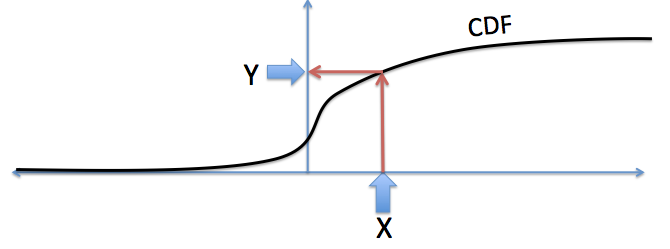
\includegraphics[width=5in]{figs/CDFmapping.png}
\end{center}
\caption{This figure depicts an example of mapping a random variable
  $X$ whose distribution is defined by a CDF (thick black curve) to
  another random variable $Y$, whose distribution is uniform in the
  interval $[0,1]$. The mapping uses the CDF as a function so that
  $Y=\CDF(X)$. \label{fig:CDFmap}}
\end{figure}

\begin{figure}[h]
\begin{center}
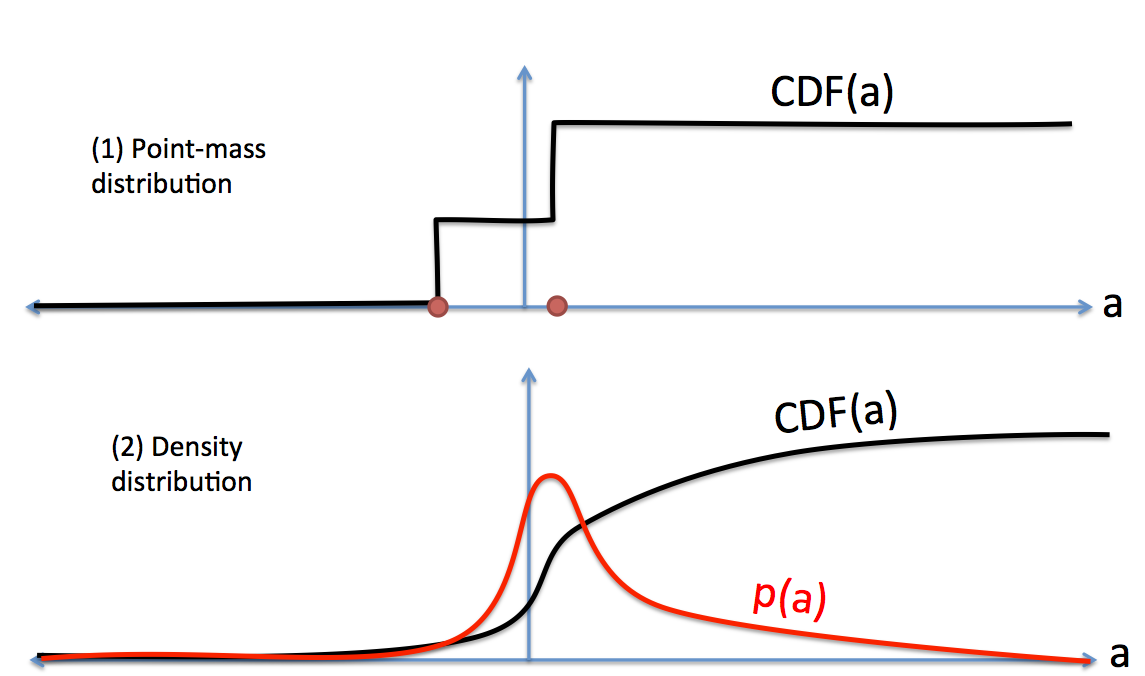
\includegraphics[width=5in]{figs/CDFs.png}
\end{center}
\caption{The CDFs for two distributions: (1) A point-mass distribution
  is a distribution that assignes non zero probabilities to two real
  values (marked by red circles) all sets that do not include at least
  one of these points have probability zero. The CDF of a point mass
  distribution is constant every where but at the point masses where
  it is discontinuous, the size of the discontinuity is the
  probability of the corresponding point. (2) A density distribution
  assigns probability zero to any single point. The CDF for such a
  distribution is a continuous increasing function that has a
  derivative. This derivative, $p(a)$ is called the {\em density function} of
  the distribution. For density distributions the CDF and the density
  function contain the same information.\label{fig:CDF}}
\end{figure}

As we see in Figure~\ref{fig:CDF} the CDF is an increasing function that
increases from zero at $-\infty$ to one at $+\infty$.

It is easy to see that $P(a<x\leq b)=\CDF(b)-\CDF(a)$.


\subsection{Examples of distributions on the real line}
If the distribution assigns a non-zero probability to some $x=a$ we
say that the distribution has a {\em point mass} at $a$. In that case
the $\CDF$ has a jump at $a$. We denote a point mass distribution
concentrated at the point $a$ by $PM(a)$. The distribution $PM(a)$
corresponds to a random variable such that $P(X=a)=1$.

\begin{figure}[t]
\begin{center}
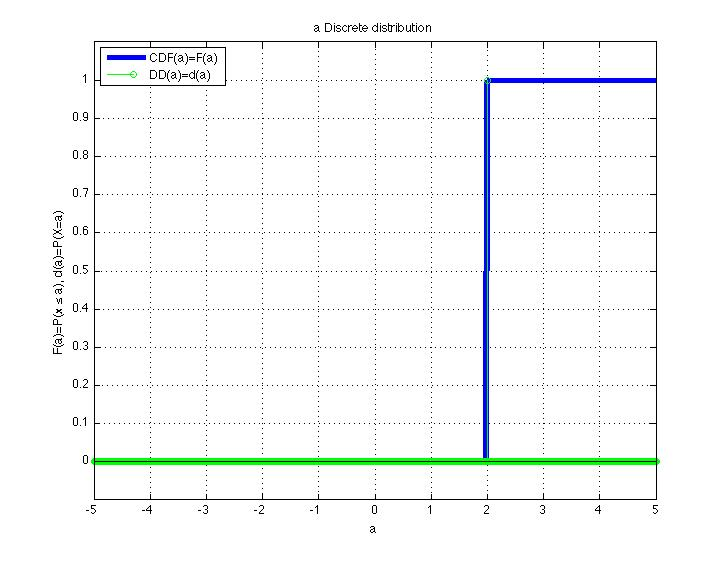
\includegraphics[width=3in]{figs/Discrete1.jpg}
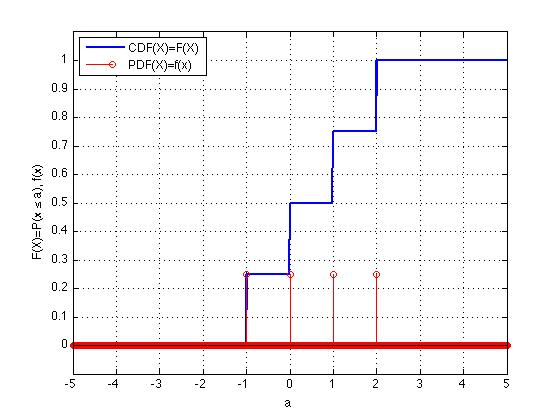
\includegraphics[width=3in]{figs/4PointMass.jpg}
\end{center}
\caption{{\bf Left:} A discrete distribution concentrated on a single
  point $P(X=2)=1$. We denote this distribution by $PM(2)$.  {\bf
    Right:} A discrete distribution distributed evenly over the four
  points $-1,0,1,2$. This distribution can be expressed as $(PM(-1)+PM(0)+PM(1)+PM(2))/4$.}
\end{figure}

\begin{figure}[b]
\begin{center}
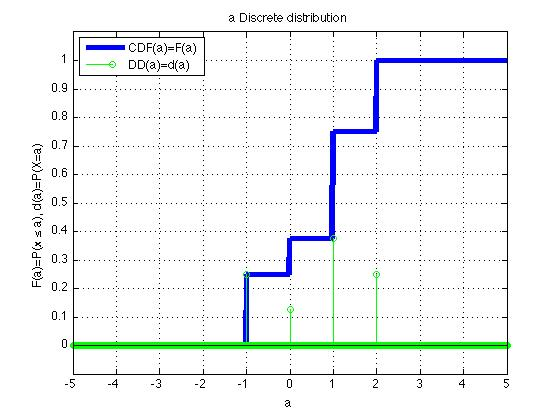
\includegraphics[width=3in]{figs/Discrete2.jpg}
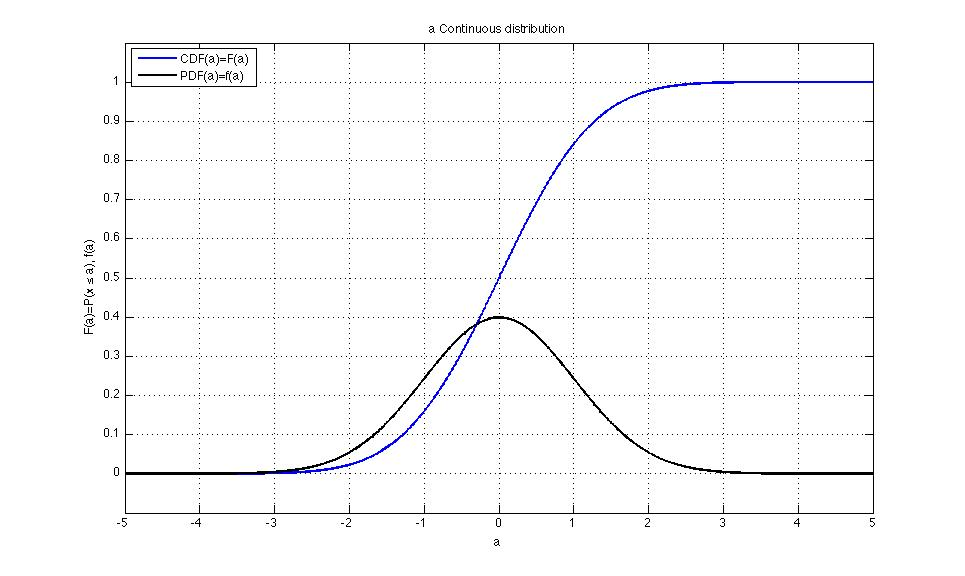
\includegraphics[width=3in]{figs/Normal.jpg}
\end{center}
\caption{{\bf Left:} A non-uniform discrete distribution. This
  distribution can be expressed as
  $(1/4)PM(-1)+(1/8)PM(0)+(5/8)PM(1)+(1/4)PM(2)$. {\bf Right:} The
  normal distribution with mean $0$ and varriance 1, denoted ${\cal
  N}(0,1)$. This is a density distribution and it's density function
is $f(x) = \frac{1}{\sqrt{2\pi}} \exp(-x^2/2)$.}
\end{figure}

\begin{figure}[t]
\begin{center}
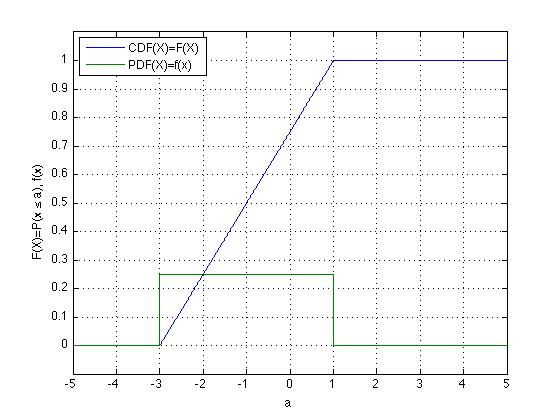
\includegraphics[width=3in]{figs/Uniform.jpg}
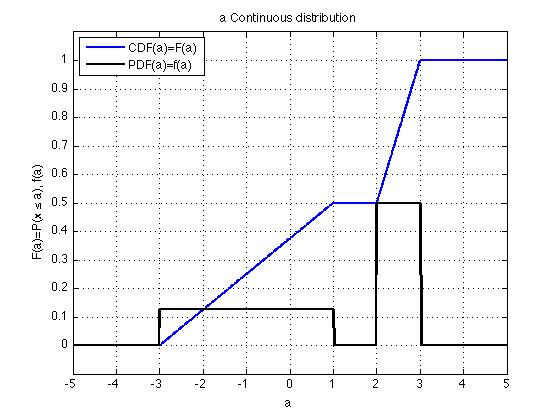
\includegraphics[width=3in]{figs/unifMixture2CDF.jpg}
\end{center}
\caption{{\bf Left:} A uniform distribution between $-3$ and $1$. We
  denote this distribution by $U(-3,1)$. {\bf Right:} A mixture of two
  uniform distributions: $(U(-3,1)+U(2,3))/2$.}
\end{figure}

\[
f(x) = \begin{cases}
0.25 & \mbox{if $ -3 \leq x \leq 1$} \\
0 & \mbox{otherwise}
\end{cases}
\]

Another important case is when the deriveative of the CDF is deifined
$p(a) = \frac{d}{dx}\left|_{x=a} \CDF(x)\right.$. The function $p(a)$
is called the {\em probability density}. Note that if $p(a)$ is
defined then, regarless of how large $p(a)$ is, $P(x=a)=0$.

When a distribution over the reals is a density distribution we can
calculate the probability of the segment $[a,b]$ using the integral:
\[
P(a < x \leq b)=\CDF(b)-\CDF(a)=\int_a^b p(x) dx
\]

\subsection{Worst-case lower bound on sorting}
You probably know of some algorithms for sorting $n$ numbers in
$O(n\log n)$ time. QuickSort and MergeSort are two such algorithms.

However, did you know that $n \log n$ is a lower bound on {\em any} sorting
algorithm? There is no sorting algorithm that can sort {\em any}
sequence of $n$ elements in time $o(n\log n)$. 

The argument is pretty simple. Let us restrict our attention to a
sequence of length $n$ that consists of the numbers $1,\ldots,n$
appearing in some order,  in other words, some permutation of the
numbers $1,\ldots,n$. As we have shown earlier in the class, there are
$n!$ such permutations.

An algorithm which sorts each of these sequences must be able to
distinguish each one of the $n!$ permutations. Suppose that the
algorithm proceeds by comparing pairs of elements in the
sequence. Each comparison has two possible outcomes. The result is a
binary tree where internal nodes correspond to comparisons and the
leaves correspond to permutations.

\begin{center}
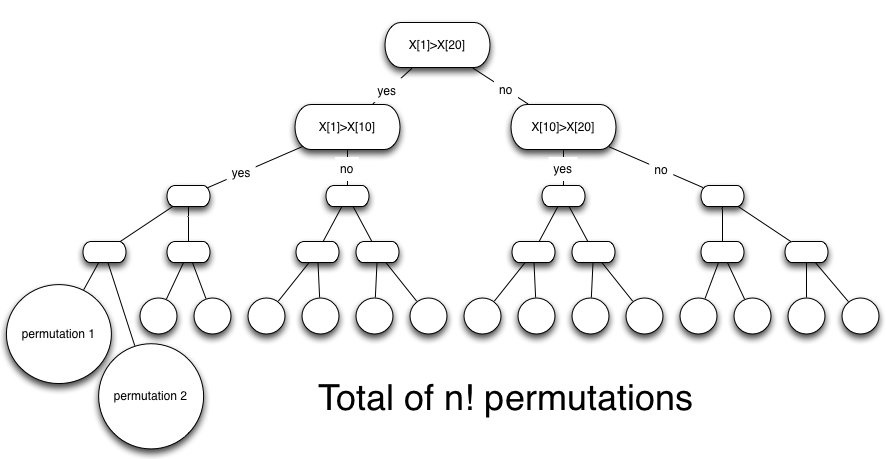
\includegraphics[width=4in]{figs/SortingLowerBound.png}
\end{center}

The depth $d$ of the tree is the worst case number of comparisons done by
the algorithm and therefor a lower bound on the worst case running
time. A basic fact about binary trees is that the number of leaves is
at most $2^d$. We there for have that $n! \leq 2^d$. Taking the
natural log of both sides and using the Strling approximation of 
$n!$ (google it!) we
find that $d \ln 2 \geq \ln n! \geq (n-1) \ln n$. We have thus found that the
worst case running time of any sorting algorithm is $\Omega(n \log n)$.

This shows that the worst case running time is $\Omega(n \log
n)$. However, as we shall see, there are sorting algorithms that,
under some statistical assumptions, take time O(n) in expectation.

\subsection{Sorting in expected linear time}

Suppose we want to sort an array of numbers $S[1\cdots n]$ that we expect to be
distributed uniformly in some range $[\min,\max]$. Here's a {\it bucket sort} approach:
\begin{itemize}
\item Divide $[\min,\max]$ into $n$ equal-sized intervals. These are the {\it buckets} 
$B_1, B_2, \ldots, B_n$.
\item Now scan array $S$ from left to right, putting each element $S[i]$ in its
appropriate bucket.
\item Return $\mbox{sort}(B_1) \circ \mbox{sort}(B_2) \circ \cdots \circ \mbox{sort}(B_n)$,
where ``sort'' is a standard sorting algorithm (say mergesort).
\end{itemize}

Notice that there is no randomization in the algorithm. However, we can talk about
the expected running time if the elements of $S$ are generated from a uniform 
distribution over $[\min,\max]$. In that case, each element is equally likely to 
fall into any of the buckets $B_i$.

Let $N_i$ be the number of array elements that fall into $B_i$. Assuming
we use a standard sorting procedure for each bucket, we get a total running time of
$$ T = N_1 \log N_1 + N_2 \log N_2 + \cdots + N_n \log N_n \ \leq \ 
N_1^2 + N_2^2 + \cdots + N_n^2 .$$

What is $\E(N_i^2)$? The easiest way to compute this is to write $N_i$ as a sum:
$$ N_i = X_1 + X_2 + \cdots + X_n$$
where $X_j$ is 1 if the array element $S[j]$ falls into bin $i$, and 0 otherwise.
Notice that $X_j^2 = X_j$, and that $X_j$ is independent of $X_{j'}$ whenever $j \neq j'$.
Therefore,
\begin{eqnarray*}
\E(X_j)  &  = & \frac{1}{n} \\
\E(X_j^2) & = & \frac{1}{n} \\
\E(X_jX_j') & = & \E(X_j) \E(X_{j'}) \ \ = \ \ \frac{1}{n^2} \mbox{\ \ \ \ if $j \neq j'$}
\end{eqnarray*}
By linearity of expectation, we then have
\begin{eqnarray*}
\E(N_i^2) 
& = & \E \left( (X_1 + \cdots + X_n)^2 \right) \\
& = & \E \left( \sum_j X_j^2 + \sum_{j \neq j'} X_j X_{j'} \right) \\
& = & \sum_j \E(X_j^2) + \sum_{j \neq j'} \E(X_j X_{j'}) \\
& = & n \cdot \frac{1}{n} + n(n-1) \frac{1}{n^2} \ \ \leq \ \ 2.
\end{eqnarray*}

So the expected running time of the sorting algorithm, once again invoking linearity, is
$$ \E(T) 
\ \leq \ \E(N_1^2) + \E(N_2^2) + \cdots + \E(N_n^2) 
\ \leq \ 2n
.$$
It is linear!

\subsection{Sorting in linear time when the distribution is known}

In the previous section we described an algorithm that can sort
elements drawn IID from the uniform distribution in expected linear
time. In this section we show how to generalize this to sorting
elements drawn IID from an arbitrary density function over the reals.

Suppose we use the CDF as a transformation, in other words, map each
$X$ to $Y=\CDF(X)$. $Y$ is a new random variable, see
figure~\ref{fig:CDFmap}. What is the distribution of the random
variable $Y$? First, it is clear that $0 \leq Y \leq 1$ because that
is the range of cumulative distribution function. We need to also
assume that the CDF is a {\em reversible} function. I.e. for any real
in the range: $0<c<1$ there exists an inverse $b=\CDF^{-1}(c)$ such
that $\CDF(b)=c$. A sufficient condition for this to hold is that the
distribution over $R$ is defined by a density function.

To understand the distribution of $Y$, let us calculate the
probability that $Y$ is in some range $c<Y<d$, where $0<c<d<1$.
Using the definition of $\CDF^{-1}$ we get
\begin{equation} \label{eqn:CDF}
P(c \leq Y \leq d) = P(\CDF^{-1}(c) \leq X \leq \CDF^{-1}(d)) =
\CDF(\CDF^{-1}(d))-\CDF(\CDF^{-1}(c)) = d-c
\end{equation}
Where the first equality is justified by the definition of
$\CDF^{-1}$, the second by the formula for calculating the probability
of a segment using the CDF, and the fourth by the cancellation :
$\CDF^{-1}(\CDF(X))=X$.  We find that the distribution of $Y$ is
uniform between 0 and 1, under the condition that the CDF is invertible.

It might help to consider a particular CDF as an example. Suppose the
CDF of $X$ is $\CDF(x) = \frac{1}{1+e^{-x}}$, this function is
invertible and it's inverse is
$\CDF^{-1}(y)=\ln\left(\frac{1}{y}-1\right)$. Apply the steps of
Equation~(\ref{eqn:CDF}) to convince yourself the it works.

Recall that we have an efficient algorithm for sorting numbers that
are distributed uniformly in some segment $[\min,\max]$.
If we know the CDF of the distribution that is generating the
numbers we wish to sort, we can map these numbers to the rannge
$[0,1]$ and then use the method suggested in the first section to sort
them in $O(N)$ time.

\section{Karger's minimum cut algorithm}

\subsection{Clustering via graph cuts}

Suppose a mail order company has the resources to prepare two different versions of 
its catalog, and it wishes to target each version towards a particular sector of its 
customer base. The data it has is a list of its regular customers, along with their 
purchase histories. How should this set of customers be partitioned into two coherent 
groups?

One way to do this is to create a graph with a node for each of the regular customers,
and an edge between any two customers whose purchase patterns are similar. The goal is
then to divide the nodes into two pieces which have very few edges between them.

More formally, the {\it minimum cut} of an undirected graph $G = (V,E)$ is a partition
of the nodes into two groups $V_1$ and $V_2$ (that is, $V = V_1 \cup V_2$ and, 
$V_1 \cap V_2 = \emptyset$), so that the number of edges between $V_1$ and $V_2$ is
minimized. In the graph below, for instance, the minimum cut has size two and partitions
the nodes into $V_1 = \{a,b,e,f\}$ and $V_2 = \{c,d,g,h\}$.

\begin{center}
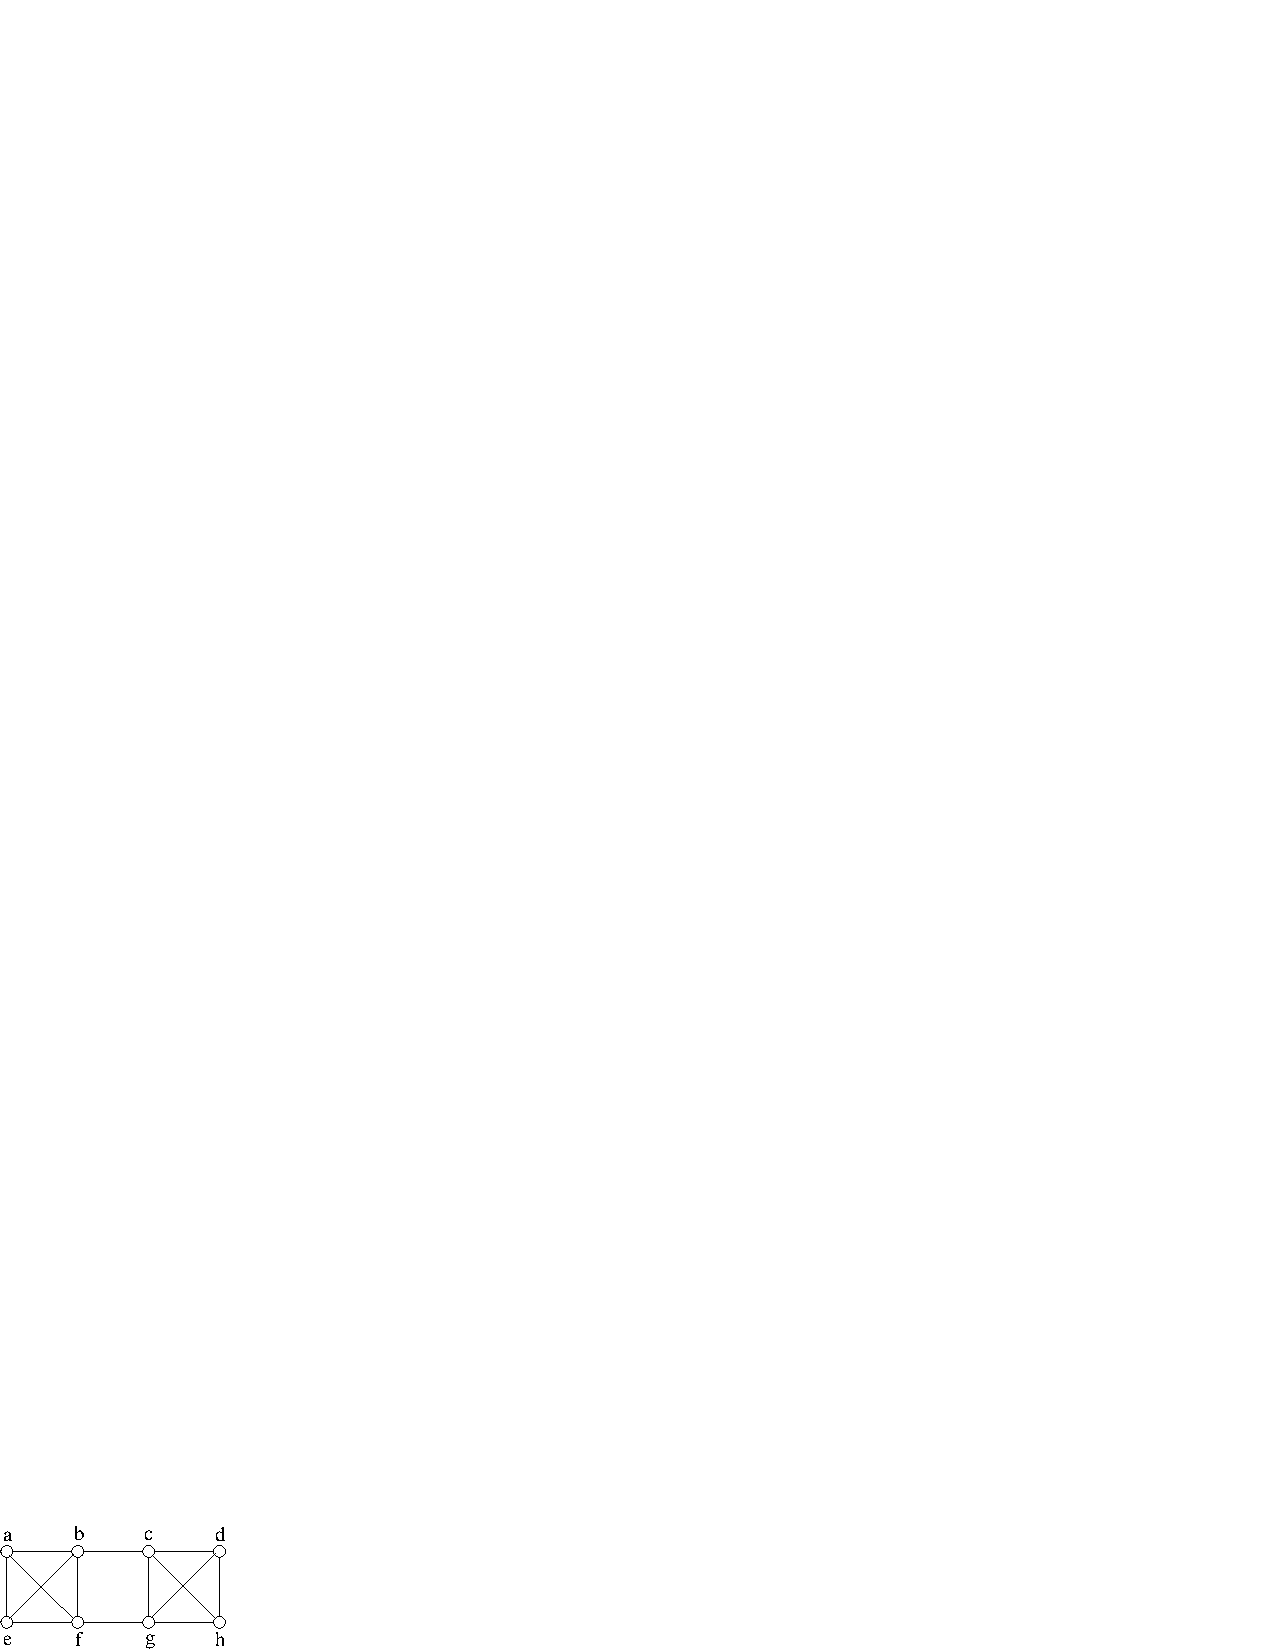
\includegraphics[width=1.5in]{figs/mincut}
\end{center}

\subsection{Karger's algorithm}

Here's a randomized algorithm for finding the minimum cut:

\begin{itemize}
\item Repeat until just two nodes remain:
\begin{itemize}
\item Pick an edge of $G$ at random and collapse its two endpoints into a single node
\end{itemize}
\item For the two remaining nodes $u_1$ and $u_2$, set 
$V_1 = \{\mbox{nodes that went into $u_1$}\}$ and 
$V_2 = \{\mbox{nodes in $u_2$}\}$
\end{itemize}
An example is shown in Figure~\ref{fig:karger}. Notice
how some nodes end up having multiple edges between them.

\begin{figure}
\begin{center}
\begin{tabular}{cp{.25in}p{2.5in}} \\ \hline

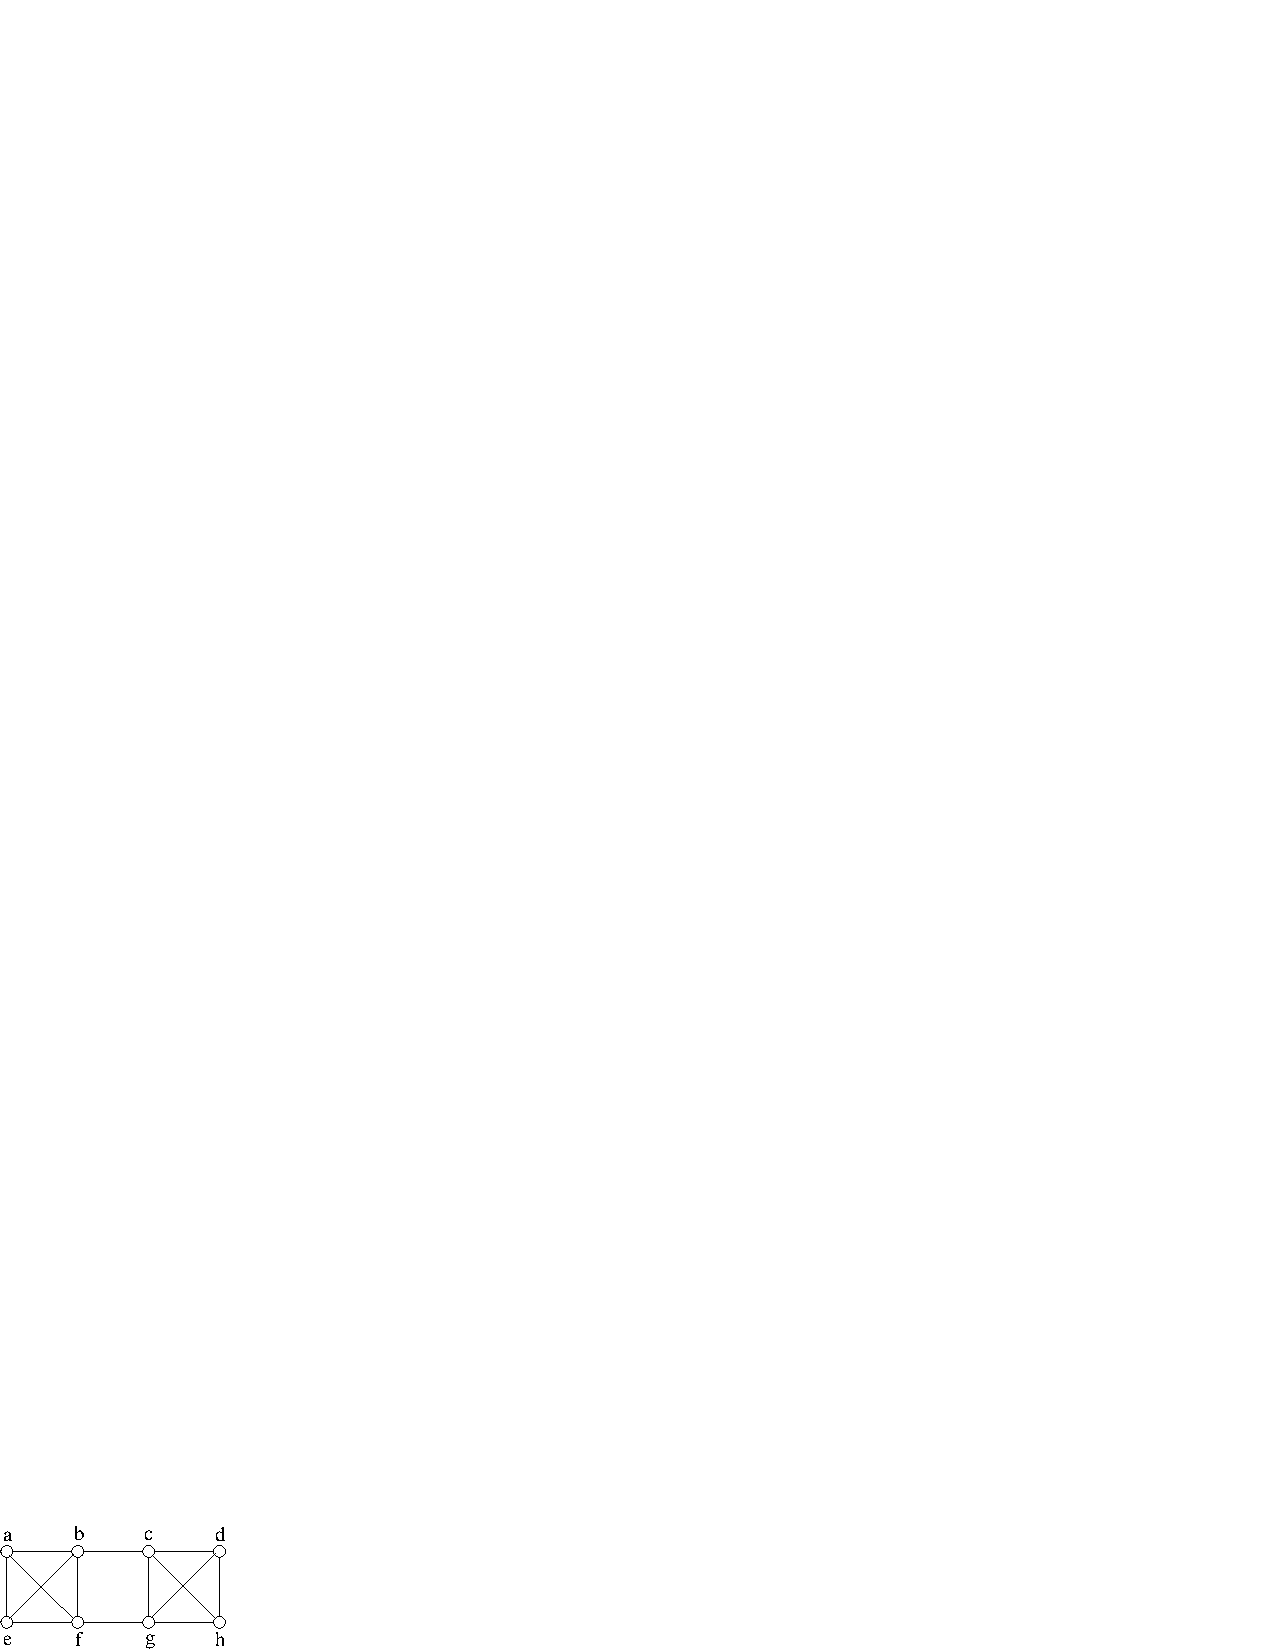
\includegraphics[width=1.5in]{figs/mincut.pdf}
&
&
\raisebox{.4in}
{\begin{minipage}[c]{2.5in}
14 edges to choose from \\
Pick $b-f$ (probability $1/14$)
\end{minipage}}
\\ \hline

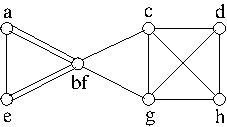
\includegraphics[width=1.5in]{figs/cut1.pdf}
&
&
\raisebox{.4in}
{\begin{minipage}[c]{2.5in}
13 edges to choose from \\
Pick $g-h$ (probability $1/13$)
\end{minipage}}
\\ \hline
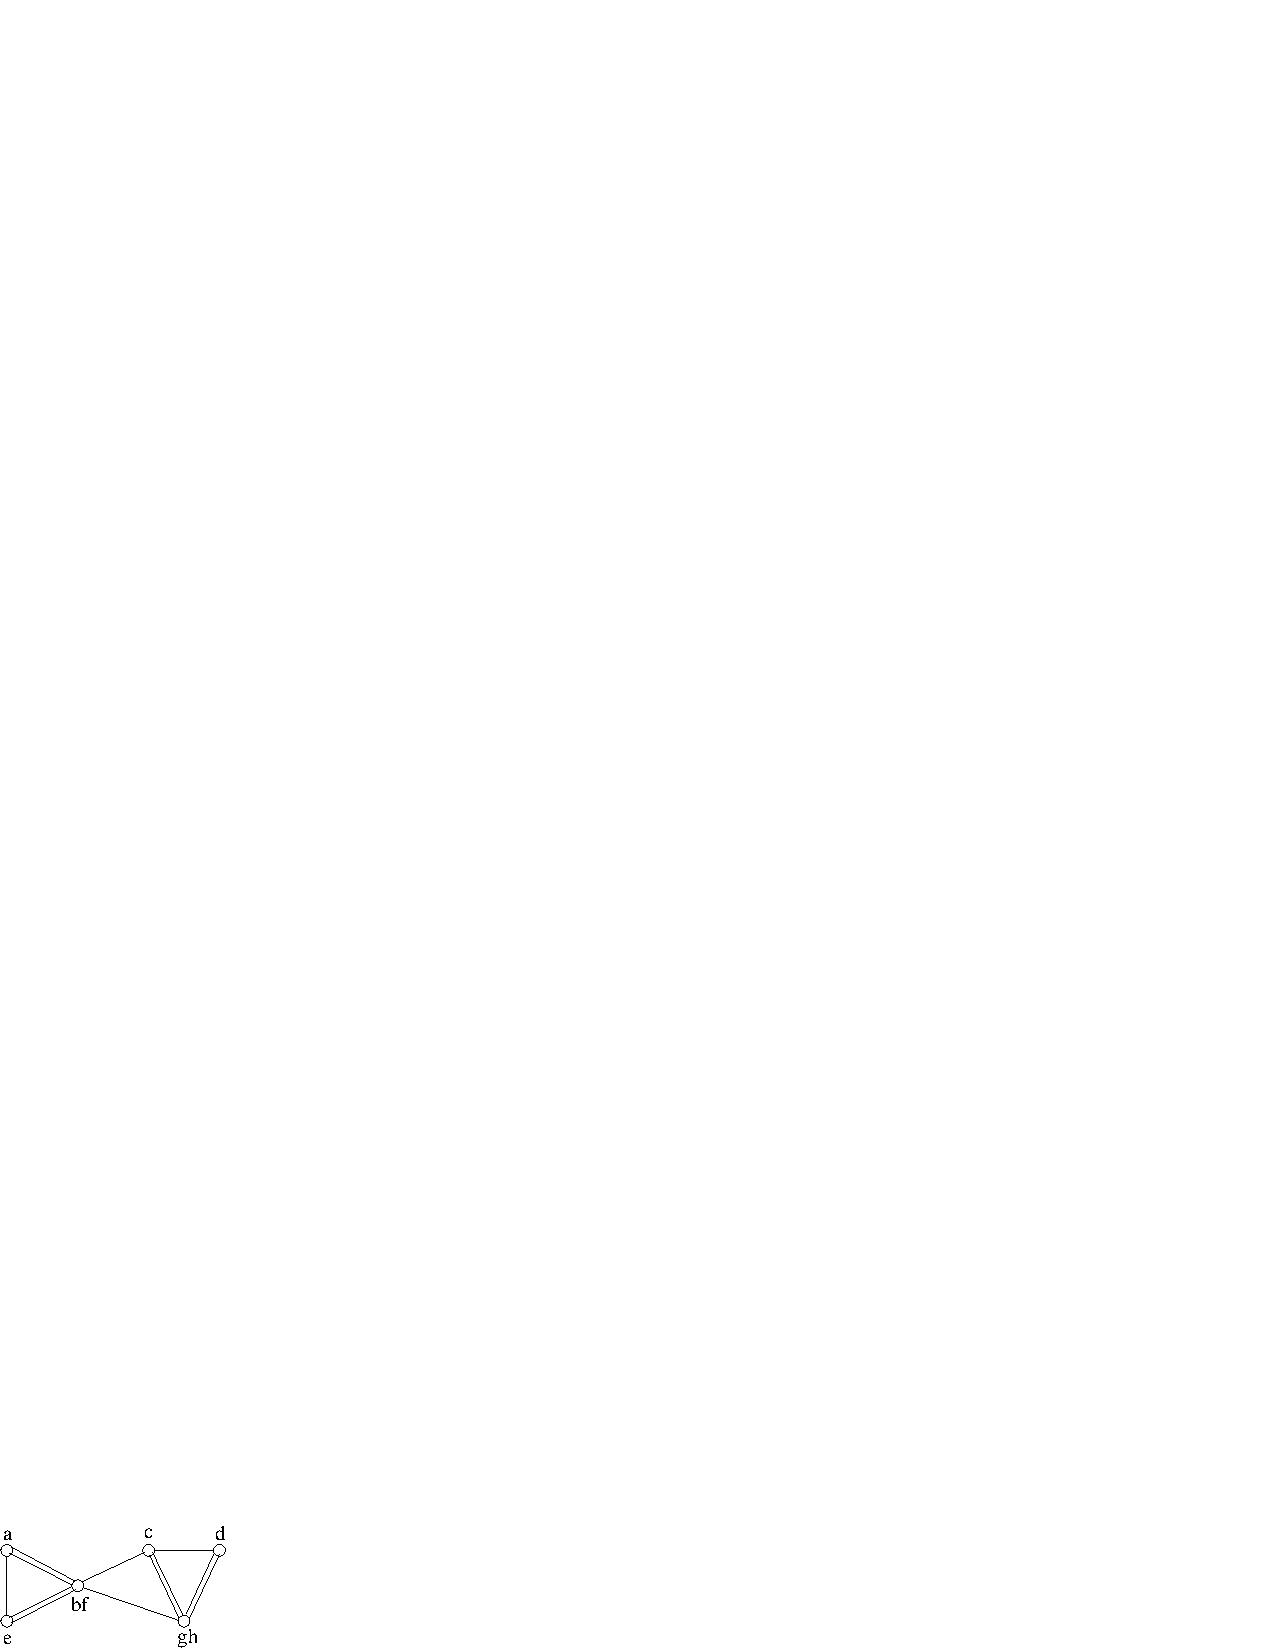
\includegraphics[width=1.5in]{figs/cut2.pdf}
&
&
\raisebox{.4in}
{\begin{minipage}[c]{2.5in}
12 edges to choose from \\
Pick $d-gh$ (probability $1/6$)
\end{minipage}}
\\ \hline

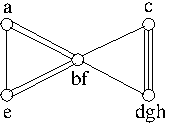
\includegraphics[width=1.25in]{figs/cut3.pdf}
&
&
\raisebox{.4in}
{\begin{minipage}[c]{2.5in}
10 edges to choose from \\
Pick $a-e$ (probability $1/10$)
\end{minipage}}
\\ \hline

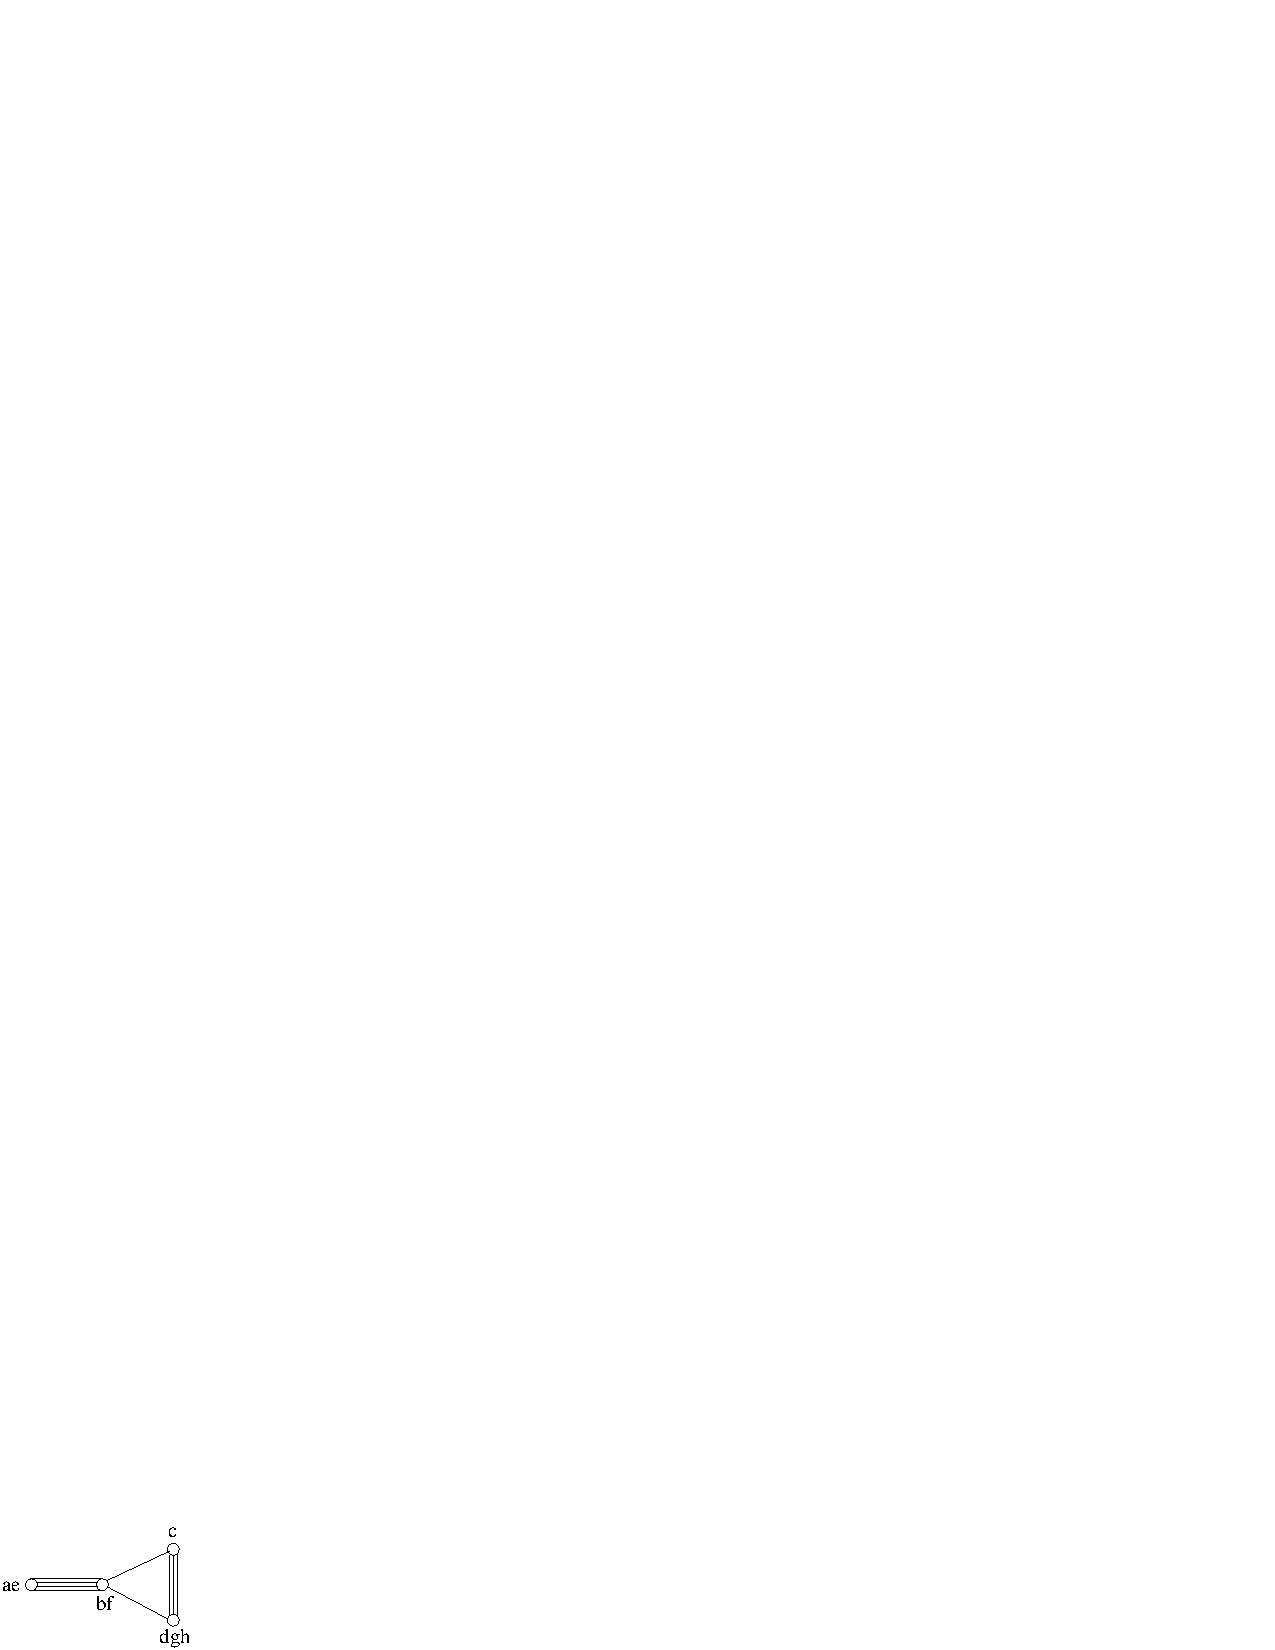
\includegraphics[width=1.35in]{figs/cut4.pdf}
&
&
\raisebox{.4in}
{\begin{minipage}[c]{2.5in}
9 edges to choose from \\
Pick $ab-ef$ (probability $4/9$)
\end{minipage}}
\\ \hline

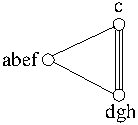
\includegraphics[width=1in]{figs/cut5.pdf}
&
&
\raisebox{.4in}
{\begin{minipage}[c]{2.5in}
5 edges to choose from \\
Pick $c-dgh$ (probability $3/5$)
\end{minipage}}
\\ \hline

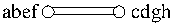
\includegraphics[width=1.25in]{figs/cut6.pdf}
&
&
\raisebox{.05in}
{\begin{minipage}[c]{2.5in}
Done: just two nodes remain
\end{minipage}}
\\ \hline
\end{tabular}
\end{center}
\caption{Karger's algorithm at work.}
\label{fig:karger}
\end{figure}



\subsection{Analysis}

Karger's algorithm returns the minimum cut with a certain probability. To analyze it,
let's go through a succession of key facts.

\begin{fact}
If $\mbox{degree}(u)$ denotes the number of edges touching node $u$, then
$$ \sum_{u \in V} \mbox{degree}(u) = 2|E|.$$
\end{fact}
To see this, imagine the following experiment: for each node, list all the edges touching 
it. The number of edges in this list is exactly the left-hand sum. But each edge appears 
exactly twice in it, once for each endpoint.

\begin{fact}
If there are $n$ nodes, then the average degree of a node is $2|E|/n$.
\end{fact}
This is a straightforward calculation: when you pick a node $X$ at random,
$$ 
\E[\mbox{degree}(X)] 
\ = \ 
\sum_{u \in V} \pr(X = u) \mbox{degree}(u) 
\ = \ 
\frac{1}{n} \sum_u \mbox{degree}(u) 
\ = \ 
\frac{2|E|}{n}
$$
where the last step uses the first Fact.

\begin{fact}
The size of the minimum cut is at most $2|E|/n$.
\end{fact}
Consider the partition of $V$ into two pieces, one containing a single node $u$, and the 
other containing the remaining $n-1$ nodes. The size of this cut is $\mbox{degree}(u)$.
Since this is a valid cut, the minimum cut cannot be bigger than this. In other words,
for all nodes $u$,
$$ \mbox{(size of minimum cut)} \leq \mbox{degree}(u) .$$
This means that the size of the minimum cut is also $\leq$ the average degree, which 
we've seen is $2|E|/n$.

\begin{fact}
If an edge is picked at random, the probability that it lies across the minimum cut is 
at most $2/n$.
\end{fact}
This is because there are $|E|$ edges to choose from, and at most $2|E|/n$ of them are
in the minimum cut.
\\

Now we have all the information we need to analyze Karger's algorithm. It returns the
right answer {\it as long as it never picks an edge across the minimum cut}. If it always 
picks a non-cut edge, then this edge will connect two nodes on the same side of the cut,
and so it is okay to collapse them together.

Each time an edge is collapsed, the number of nodes decreases by 1. Therefore,
\begin{eqnarray*}
\pr(\mbox{final cut is the minimum cut})
& = &
\pr(\mbox{first selected edge is not in mincut}) \times \\
& & \pr(\mbox{second selected edge is not in mincut}) \times \cdots \\
& \geq & 
\left( 1 - \frac{2}{n} \right) \left( 1 - \frac{2}{n-1} \right) 
\left( 1 - \frac{2}{n-2} \right) \cdots \left( 1 - \frac{2}{4} \right) 
\left( 1 - \frac{2}{3} \right) \\
& = & 
\frac{n-2}{n} \cdot \frac{n-3}{n-1} \cdot \frac{n-4}{n-2} \cdots \frac{2}{4} \cdot 
\frac{1}{3} \\
& = & 
\frac{2}{n(n-1)} .
\end{eqnarray*}
The last equation comes from noticing that almost every numerator cancels with the 
denominator two fractions down the line.

Karger's algorithm succeeds with probabililty $p \geq 2/n^2$. Therefore,
it should be run $\Omega(n^2)$ times, after which the smallest cut found should
be chosen.

Those who are familiar with minimum spanning tree algorithms might be curious to
hear that another way to implement Karger's algorithm is the following:
\begin{itemize}
\item Assign each edge a random weight
\item Run Kruskal's algorithm to get the minimum spanning tree
\item Break the largest edge in the tree to get the two clusters
\end{itemize}
(Do you see why?) Over the decades, the running time of Kruskal's algorithm has 
been thoroughly optimized via special data structures. Now this same technology 
can be put to work for cuts!

\section{Hashing}

In many situations, such as a dictionary application, we need to store a vast 
collection of items in such a way that we can look up any item instantaneously. 
The way to do this is by {\it hashing}.

\subsection{The hashing framework}

Suppose you have a large collection of items $x_1, \ldots, x_n$ that you want 
to store (for instance, all English words), where these items are 
drawn from some set $\U$ (for instance, the set of all conceivable words). 
The requirements are:
\begin{enumerate}
\item The total storage space used should be $O(n)$.
\item Given a query $q \in \U$, it should be possible to {\it very rapidly}
determine whether $q$ is one of the stored items $x_i$.
\end{enumerate}

\subsection{A simple solution using randomization}

\begin{enumerate}
\item Pick a completely random function $h: \U \rightarrow \{1,2,\ldots, n\}$. 

This is the {\it hash function}. 

\item Create a table $T$ of size $n$, each of whose entries is a pointer to a 
linked list, initialized to null. 

\item Store each $x_i$ in the linked list at $T[h(x_i)]$.

We say $x_i$ {\it hashes to} location $h(x_i)$.

\item Given a query $q$, look through the linked list at $T[h(q)]$ to see if
it's there.
\end{enumerate}

Here's a picture of the data structure.

\begin{center}
%%\resizebox{2.25in}{!}{\input{figs/table.pstex_t}}
\end{center}

The storage used is $O(n)$. What about the query time?

\subsection{Average query time}

Suppose query $q$ is picked at random, so that it is equally likely to hash to
any of the locations $1,2,\ldots, n$. What is the expected query time?
\begin{eqnarray*}
\mbox{Expected query time}
& =& 
\sum_{i=1}^n \pr(\mbox{$q$ hashes to location $i$}) \cdot \mbox{(length of list at $T[i]$)} \\
& =&
\frac{1}{n} \sum_i  \mbox{(length of list at $T[i]$)} \\ 
& = & 
\frac{1}{n} \cdot n \ = \ 1
\end{eqnarray*}
So the average query time is constant!

\subsection{Worst case query time, and a balls-in-bins problem}

What is the worst case query time; that is, what is the length of the
longest linked list in $T$? Equivalently, when you throw $n$ balls in
$n$ bins, what is the size of the largest bin? We'll see that with
very high probability, no bin gets $\geq \log n$ balls.

For any bin $i$, let $E_i$ be the event that it gets $\geq \log n$ balls.
$$ \pr(E_i) \  \leq \ {n \choose \log n} \left( \frac{1}{n} \right)^{\log n} .$$
(Do you see why?) 

To upper bound this probability we use the inequality (see cheat sheet) that
\[
{n \choose k} \leq \left( \frac{ne}{k} \right)^k
\]
Applying this inequality we get:
\[
{n \choose \log n} \left( \frac{1}{n} \right)^{\log n} \leq 
\left( \frac{ne}{n \log n}  \right)^{\log n} =
\left( \frac{e}{\log n}  \right)^{\log n} =
\frac{n^{\log e}}{(\log n)^{\log n}} \leq \frac{1}{n^2}
\]
Where the last inequality can be shown by moving the $n$ from the left
to the right and taking $1/x$ and then log of both sides:
\[
(\log n)(\log \log n) \geq (2+\log e) \log n
\]
Which holds when $n>2000$

Having shown that $\pr(E_i) \leq 1/n^2$, it follows that
$$ \pr(\mbox{some bin gets $\geq \log n$ balls})
\ = \ 
\pr(E_1 \cup E_2 \cup \cdots \cup E_n)
\ \leq \ 
\pr(E_1) + \cdots + \pr(E_n) 
\ \leq \ 
\frac{1}{n}.
$$
For instance, if you throw a million balls into a million bins, then the chance that
there is a bin with $\geq 20$ balls is at most 1 in a million.

Getting back to hashing, this means that the worst case query time is (with high
probability) $O(\mbox{log} n)$.

\subsection{The power of two choices}

Here's a variant on the balls and bins setup. As usual, you have before you a 
row of $n$ bins, along with a collection of $n$ identical balls. But now, 
when throwing each ball, {\it you pick two bins at random and you put the
ball in whichever of them is less full}.

It turns out, using an analysis that is too complicated to get into here, that
under this small change, the maximum bin size will be just $O(\log \log n)$ 
instead of $O(\log n)$.

This inspires an alternative hashing scheme:

\begin{enumerate}
\item Pick {\it two} completely random functions $h_1, h_2: \U \rightarrow \{1,2,\ldots, n\}$. 

\item Create a table $T$ of size $n$, each of whose entries is a pointer to a 
linked list, initialized to null. 

\item For each $x_i$, store it in either the linked list at $T[h_1(x_i)]$ or $T[h_2(x_i)]$,
whichever is shorter.

\item Given a query $q$, look through {\it both} the linked list at $T[h_1(q)]$ and
at $T[h_2(q)]$ to see if it's there.
\end{enumerate}

The storage requirement is still $O(n)$, the average query time is still $O(1)$, but now
the worst case query time drops to $O(\log \log n)$.

\section{Information retrieval}

When you go to Google and enter a query, like
\begin{quote}
{\tt what are treatment options for pneumonia}
\end{quote}
or
\begin{quote}
{\tt new song by radiohead}
\end{quote}
you immediately get back a list of highly suitable pages. It's as if the search engine
were instantaneously able to look through the tens of billions of pages on the web and
find the relevant ones. How does it pull this off? The answer is, by a combination of
clever preprocessing, statistics, hashing, and clustering.

In fact, these basic techniques apply not just to web search but to any system for
{\it information retrieval}: answering unstructured queries about a large collection
of documents.

\subsection{Preprocessing}

There are at five crucial preprocessing steps for a search engine.
\begin{enumerate}
\item Give each webpage a {\it reliability score}.

Most of the ``information'' on the web is grossly unreliable: spam, ignorant ravings, unfounded conjectures, and idle gossip. But we'll see (a bit later in the course) that it is possible to assess the reliability or authoritativeness of individual webpages --- by analyzing the statistics of linkage patterns.

\item Ignore {\it near-duplicates} of webpages.

More on this very shortly.

\item Discover the set of {\it terms}.

A {\it term} is an individual word, or a sequence of words that should be considered together, such as {\tt Katy Perry} or {\tt Rage Against the Machine}. Terms can be discovered by analyzing co-occurrence patterns. If a sequence of $k$ words keeps occurring together, they should be designated a term.

\item Create the {\it postings list}.

This is a hash table in which each term is associated with a linked list of the pages containing it.

\begin{center}
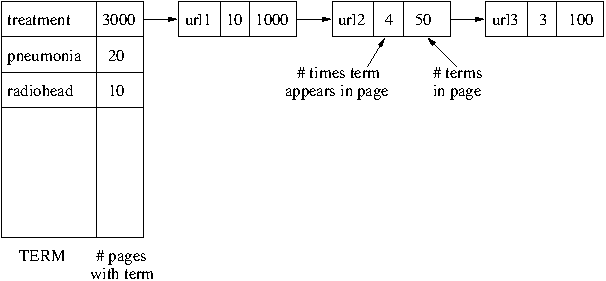
\includegraphics[width=5in]{figs/postings.pdf}
\end{center}

Each linked list is arranged in decreasing order of ``priority'' (some notion that takes into account reliability scores), and is usually truncated at a certain point.

\item Compute {\it term frequencies}.

How common is each term?

\end{enumerate}

\subsection{Answering a query}

The first step in answering a query is to order query terms by importance. The important terms are those that are uncommon. For instance, in
\begin{quote}
{\tt what are treatment options for pneumonia}
\end{quote}
the most important term is {\tt pneumonia}, since this is the least common. Next comes {\tt treatment}, and then {\tt options}. The remaining words are so common that they can be ignored.

The next step is to look at the postings list, and get all pages containing the important query term(s). Then, assign each a score based on:
\begin{itemize}
\item the reliability of that page
\item which of the important query terms it contains
\item the number of times each query term appears on that page, divided by the length of the page
\end{itemize}

This yields an ordered list of webpages, starting with the ``most relevant''. But the list will typically contain way too many pages. So they need to be clustered, and the user can then be presented with one representative page from each cluster, with the option to select ``more like this''.

For instance, pages about {\tt Rome} might be clustered into categories based on whether they refer to:
\begin{itemize}
\item Ancient Rome
\item Modern Rome
\item The TV series ``Rome''
\item and so on.
\end{itemize}

\section{Detecting near-duplicates}

Near-duplication is pervasive in the web: there are large numbers of distinct URLs which have exactly
the same content but differ only in unimportant details like headers and footers. The user of a search
engine would not be pleased if the answer to his query was a set of 10 near-identical pages! In order
to remove this redundancy, we need to define a notion of {\it similarity} between documents.

\subsection{The similarity between two documents}

For any document---call it $d$---let the set of all words in $d$ be denoted $C(d)$. For two documents 
$d$ and $d'$, we will measure their similarity by the function
$$ S(d,d') \ = \ \frac{|C(d) \cap C(d')|}{|C(d) \cup C(d')|} .$$
If the two documents are truly identical, $S(d,d') = 1$. If they are almost-identical, $S(d,d')$ will
be close to 1. And if they are completely different, with no words in common, then $S(d,d')$ will be
zero. We'll consider $d$ and $d'$ to be near-duplicates if $S(d,d')$ is sufficiently close to 1.

Now, imagine a search engine that is going through a list of documents or webpages, and wants to 
eliminate near-duplicates. Here's an algorithm it could use:
\begin{itemize}
\item ${\cal D} = \emptyset$ (set of documents, initially empty)
\item for each document $d$ that appears:
\begin{itemize}
\item if $S(d,d')$ is significantly smaller than 1 for all $d'$ in ${\cal D}$: add $d$ to ${\cal D}$
\end{itemize}
\end{itemize}
The final set of documents ${\cal D}$ will contain no near-duplicates. This is good, but the
algorithm is very slow. Suppose for the sake of simplicity that there are $n$ documents in total,
each of length $L$. Then computing the similarity between two documents takes $O(L)$ time, and
the algorithm is $O(n^2L)$. This quadratic dependence on $n$ is prohibitive in web-scale applications,
where $n$ could easily be in the billions or tens of billions.

To get a faster algorithm, we once again resort to hashing.

\subsection{An algorithm based on random permutations}

We will encode each document by a single number. Here's how.
\begin{itemize}
\item Pick any encoding of words as numbers: for instance, any word is in any case stored
as a binary number in the computer, and we can just use that number. Let $e(w)$ be the encoding
of word $w$. Suppose these encodings are in the range $1,\ldots, M$.
\item Let $\sigma$ be a {\it random permutation} of $(1,2,\ldots, M)$. Thus for each $i$, 
$\sigma(i)$ is a number in the range 1 to $M$, and all the $\sigma(i)$ are different.
\item Hash each document $d$ to the single number
$$ f(d) = \min \{\sigma(e(w)): w \in d\} .$$
That is, first think of all the words in the document as numbers, then apply the random 
permutation to each of these numbers (to get a different set of numbers), and finally pick
the smallest of these resulting numbers. It is important that the same permutation $\sigma$
is used for {\it all} the documents.
\end{itemize}

We will use the single number $f(d)$ in place of the entire document $d$! The rationale for doing 
this is captured in the following lemma, which says that near-duplicate documents are likely to
be hashed to the same value.
\begin{lemma}
Let $d,d'$ be any two documents. If $\sigma$ is a random permutation, then
$$ \pr(f(d) = f(d')) \ = \ S(d,d') .$$
\end{lemma}
\begin{proof}
For any word $w$, we will call $\sigma(e(w))$ its {\it value}.

Now, $f(d)$ and $f(d')$ will be equal if and only if the word in $d$ with the
smallest value is the same as the word in $d'$ with the smallest value. This is the same 
as saying that the smallest value among words in $d \cup d'$ lies in $d \cap d'$. The 
probability of this is exactly
$$ \frac{\mbox{\# words in $d \cap d'$}}{\mbox{\# words in $d \cup d'$}} \ = \ S(d,d').$$
Reason: $\sigma$ is a random permutation, so each word in $d \cup d'$ is equally likely to 
be the one with the smallest value.
\end{proof}

Here's the revised algorithm.
\begin{itemize}
\item Create a boolean array ${\tt seen}[1\ldots M]$, initialized to ${\tt false}$
\item ${\cal D} = \emptyset$ (set of documents, initially empty)
\item for each document $d$ that appears:
\begin{itemize}
\item if not ${\tt seen}[f(d)]$: add $d$ to ${\cal D}$ and set ${\tt seen}[f(d)] = {\tt true}$
\end{itemize}
\end{itemize}
This time, the running time is $O(nL)$, just linear in $n$.
\\

In practice, this algorithm is run not with the words in each document but with all 
sequences of $k$ words (called ``$k$-shingles''). For instance, the document
\begin{quote}
the quick brown fox jumped over the lazy dog
\end{quote}
has the following 3-shingles: {\tt the quick brown}, {\tt quick brown fox}, {\tt brown fox 
jumped}, {\tt fox jumped over}, {\tt jumped over the}, {\tt over the lazy}, {\tt the lazy dog}.

\section{Bloom Filters}

In some situations we are given a very long string, say billions of
characters long, and we want to find all words that appear more than
one time. A reasonably efficient way of doing that is to create a large hash
table, keyed by words which stores the {\em count} for each
observed word.  This gives us a linear time algorithm in the length of
the input. 

However, in many cases the number of different words that appear in
the input is very large but most of them occur only once
(mis-spellings, people's names etc). This single-occurance words or
{\em singletons} place a large demand on the computer memory while
containing no useful information.\footnote{ Distributions where a
  significant fraction of the items (words) in a random sample appear
  only once, are called Zipf distributions.  Zipf distributions are
  prevalent whenever a very large and under-utilized set of labels is
  used. This includes words, URLs, IP addresses etc.  You can think of
  Zipf distributions as lying in the mid-point between discrete
  distributions (over a finite set) and density distributions. In the
  first case we expect {\em all} values to appear many times in a
  large enough sample, while in the second case we don't expect to see
  {\em any} value more than once.}

What we need is a {\em filter}. This filter will recieve as input the
stream of words, one word at a time. For each word it will answer the
question ``did this word appear earlier in the stream?''. If this is
the first time the word appears, then it is {\em filtered out} or
ignored. If the word has appeared earlier then it is {\em filtered in}
or passed on to the hash table holding the counters. We would like to
find a method which uses much less memory than would be used by the
hash table.  {\bf Bloom filters} provide an elegant solution to this
problem, but with a slight caveat: while no word that appears more
than once will be mistakenly filtered out, the method does allow a
small fraction of the singletons to be filtered in.

We now describe Bloom filters. Initially, two integer parameters $k,m$
are chosen (how to choose it will be described a little later). We
then choose and fix $k$ different hash functions $h_1,h_2,\ldots,h_k$
that map words to integers in the range $1,\ldots,l$. We also allocate
a bit vector $B[\cdot]$ of length $m$ where all bits are initialized to
zero.

The filter operates as follows. Given a word $w$, it computes the $k$
numbers $h_1(w),h_2(w),\ldots,h_k(w)$ and uses them as indices into
the bit vector $B$. If all of the $k$ bits
$B[h_1(w)],B[h_2(w)],\ldots,[h_k(w)]$ are equal to 1 then the we
declare that word $w$ did appear earlier in the stream and therefor
$w$ is filtered {\em in}.  If any of the $k$ bits is not 1 then the
word $w$ is filtered {\em out} and not counted and the $k$ bits in $B$
are set to 1.

We now want to analyze the probability that the Bloom filter makes a
mistake. There are two types of mistakes: filtering out a word that
appeared previously and filtering in a word that did not appear
previously. We consider each error type in turn:
\begin{itemize}
\item {\bf Filtering out a word that appeared previously} (false
  negative) This can never happen. If the word $w$ appeared in the
  past then the bits $B[h_1(w)],B[h_2(w)],\ldots,[h_k(w)]$ have been
  set to 1. As the algorithm never resets bits to zero, these bits
  must still be all 1 when we encounter $w$ for the second, third,
  ... time. As a result $w$ will not be filtered out. The Bloom filter
  does not make false negative mistakes.
\item {\bf Filtering in a word that did not previously appear} (false
  positive) This can happen. The $k$ bits that are checked might have
  been set to 1 as a result of observing other words. However, we will
  now show that the probability of this event is small (provided $k$
  and $m$ are set appropriately. Note also that the cost of a false
  positive mistake is small - it means that the algorithm will
  unneccesarily store a singleton word in the hash table. The result
  is a waste of memory space but not an actual error.
\end{itemize}

  We now analyze the probability of making a false positive mistake,
  i.e. incorrectly declaring that a new word appeared earlier in the
  sequence. Let $n$ be the number of different elements (words) that
  we inserted into the filter before we test the new word. We assume
  that each hash function $h_j(w)$ is a number chosen uniformaly at
  random from the range $1 \leq i \leq m$. Consider a particular
  location $j$ in the bitvector $B$, which is one of the $k$ locations
  that the new word $w$ is mapped to. We want to compute the
  probability that this bit is {\em not} set to one. The probability
  that one of the $k$ hash functions, operating on one of the previous
  $n$ words, does {\em not} set the bit to one is
  \[
  1-\frac{1}{m}
  \]
  Thus the probability that none of the $k$ hash functions, operating
  on any of the $n$ words sets the $j$th bit to one is
  \[
  \left(  1-\frac{1}{m} \right)^{kn}
  \]
  Thus the probability that the $j$th bit is set to one is 
  \[
  1-\left(  1-\frac{1}{m} \right)^{kn}
  \]
  Finally, the new word will be identified as new only if all of the
  $k$ locations in $B$ to which it is hashed have been set to one. As
  these locations are independent, we get that the probability of
  making a false positive mistake is 
  \[
  \left(  1-\left(  1-\frac{1}{m} \right)^{kn} \right)^k =
  \left(  1-\left( \left(  1-\frac{1}{m} \right)^m \right)^{kn/m}\right)^k \approx
  \left(  1-e^{-kn/m}\right)^k
  \]

Note that the only way that $m$ and $n$ enter the equation is through
the ratio $m/n$. We call the ratio $r=m/n$ the {\em redundancy} of the
bitmap, because it defines the number of bits that are associated with
each word. And we can rewrite the (approximate) probability of a false 
positives as
\[
\left(  1-e^{-k/r}\right)^k
\]
The number of hash functions $k$ that approximately 
minimizes the probability is (remember that $k$ is an integer)
\begin{equation} \label{eqn:optimal-k}
k \approx r \ln 2 \approx 0.7 r
\end{equation}
which gives the false positive probability of
\[p=\left(  1-e^{-\ln 2} \right)^k = (1/2)^{k} \approx (0.6185)^{r}.\] 

The required redundancy for a desired false positive probability $p$
(assuming the optimal value of $k$ is used) can be computed by
taking the ln f the two side in the last expression
\begin{equation} \label{eqn:optimal-p}
\ln p = -r (\ln 2)^2.
\end{equation}

Recalling  that $r=m/n$ we get that the length of the bit vector is
\[m=-\frac{n\ln p}{(\ln 2)^2}.\]

To gain some intuition about these results, lets compare the
performance for the optimal $k\approx m/n$ defined in
Equation~(\ref{eqn:optimal-k}) with the performance for $k=1$.  The case
$k=1$ is very intuitive, each word is mapped to a single bit and if
this bit is one, then the algorithm concludes that the word has been
seen before. As the length of the bit vector $B$ is $m$ and the number
of different words already observed is $n$ then $n$ of the $m$ bits in
$B$ are set. The result is that the probability of making a false
positive mistake is $p=n/m$. If we had a perfect hashing
function, that maps each word to a different bit, we would be able to
use a table with no reducdancy, i.e. $r=1$. As we showed above when
$k=1$, $p=1/r$.

Condider now using the optimal setting for $k$ as defined in
Equation~(\ref{eqn:optimal-k}). In this case we have from
Equation~(\ref{eqn:optimal-p}) that:
\[
p = \exp\left( -\frac{m}{n} \left(\ln 2\right)^2 \right) \leq
    \exp\left( -0.48 \frac{m}{n} \right)
=  \exp\left( -0.48 r \right)
\]
We find that in both cases the probability of a false positive is a
function of the redundancy, however, while for $k=1$, $p$ decreases
like $1/r$ for the optimal value of $k$ it decreases much faster, like $e^{-r}$.
Thus with the same size bit vector we get a much smaller probability
of error.

\end{document}



